\documentclass{article}
\usepackage{amsmath, amssymb, graphicx, algpseudocode}
\usepackage[margin=0.5in]{geometry}

\graphicspath{images/}

\begin{document}

\title{Neural Networks}
\author{Piyush Patil}
\maketitle

\section{Introduction}
Neural networks are models that are loosely based on the topology of the human brain, and tie together several different ideas (e.g. perceptrons, logistic regression, stochastic gradient descent, etc.). Neural networks are essentially layers of perceptrons connected to each other, so the output of one perceptron becomes the input to another. Recall that perceptrons are merely very simply linear classifiers: a perceptron $ p $ is defined
$$ p(x) = \begin{cases}
    1, &\text{ if } w^\intercal x > \beta \\
    -1, &\text{ otherwise }
\end{cases} $$
$ w $ and $ \beta $ are parameters here, controlling the separating hyperplane of $ p $; the key difference between perceptrons and other linear classifiers is that perceptrons learn the optimal separating hyperplane over time, starting with a random hyperplane determined by random $ w, \beta $ and adjusting it every time a data point is seen, with adjustments depending on if the classification of the data point was correct or not. We consider each of these perceptrons as basic processing units of a connectionist system that is the neural network. Viewing perceptrons as "neurons", the idea of putting layers of perceptrons into a directed graph topology was inspired by the connectionist nature of the brain, which is itself a network of basic processing units (i.e. biological neurons) where the output of one neuron becomes the input to another. 
\newline \newline
Of course, merely stringing together several perceptrons in any configuration results in nothing more than a linear combination of compositions of more linear combinations, which will still be confined to linearly separable data. In order to extend neural networks beyond this restriction, we need to introduce a non-linearity at some point in the composition. Again turning to biology, neurons in the brain use action potentials to communicate, but the electrical impulse is only "outputted" if the neuron is "activated", which depends on some stimulus, usually the action potentials received by the neuron along dendrites, exceeding a threshold. Borrowing this idea, we might have the perceptrons compute their linear combination as usual, and then pass the linear combination through a non-linear \textit{activation function} before outputting it. Common choices of activation functions are the step function, based on some threshold (analogous to biological neurons) or the logistic function, which is a smooth version of the step function. Moreover, the firing rate of a neuron is also used as an indicator for the "strength" or magnitude of the output of the neuron; the firing rate is bounded below by 0 times per second and above by approximately 1000 times per second, so the logistic functions are good analogs for this aspect of biological neuronal outputs.

\section{Architecture}
The most common and simple neural network architecture is the \textit{feedforward} neural network, in which the network topology consists of $ L $ layers of separate, unconnected neurons; each neuron in layer $ l $ is connected to every neuron in layer $ l + 1 $. The key idea is that every neuron has parameters $ w, \beta $ associated with it, and, being a perceptron, receives as input the outputs of every neuron in the previous layer. The first layer receives as input a feature vector $ x_i $, and the last layer outputs our approximation of $ y_i $. These are, unsurprisingly, known as the \textit{input layer} and \textit{output layer}, respectively; additional layers in between are called \textit{hidden layers}.

\begin{center}
    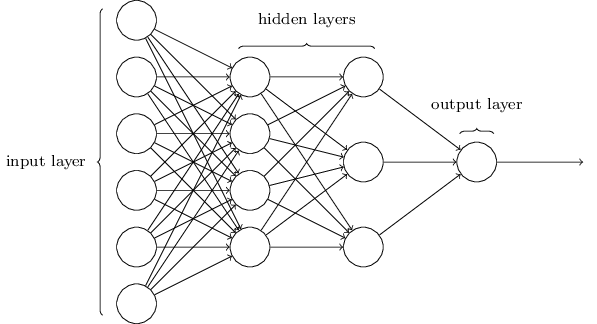
\includegraphics[scale=0.5]{images/neural_network.png}
\end{center}    

The simplest neural network is meant to be only two layers long, just an input and an output layer; this is the simplest way to compose perceptrons together - one perceptron per input in the input layer, one perceptron per output in the output layer, and a fully connected set of weights in between. The purpose of putting hidden layers in between is so the network can learn new features on its own, rather than manually construct new features to lift the data to as we did with linear classifiers. By adding more hidden layers, the network can learn its own higher level features.
\newline
The neuron treats the outputs of the neurons in the previous layer as its own feature vector, and, putting the outputs $ x_i $ into a vector $ x $, computes $ w^\intercal x + \beta $, passes it through the activation function, and sends the resulting output to every neuron in the next layer. Thus, we can recursively describe the output of neuron $ i $ in layer $ l $, denoted $ o_i^l $, with
$$ o_i^l = s \left( \sum_j w_j o_j^{l - 1} + \beta \right) $$
where $ j $ runs over the neurons in the previous layer and $ s $ is the activation function. Or, letting $ o_l $ be the vector containing the outputs of layer $ l $, $ W_l $ be the matrix containing the weights of neuron $ i $ in layer $ l $ in its $ i^{\text{th}} $ column, and $ \beta_l $ be the vector containing the shifting terms of the neurons in layer $ l $, we can write more compactly
$$ o_l = s(W_l o_{l - 1} + \beta_l) $$
where $ s $ is applied element-wise. The introduction of the non-linear activation function and the given feedforward architecture so far have been inspired by very non-rigorous, hand-wavy notions so far, and are only loosely based on the initial perceptron classifier. However, the following celebrated result explains the interest behind neural networks.
\newline \newline
\textbf{(Theorem) Cybenko's Theorem}: \textit{Also known as the \textbf{universal approximation theorem}, this theorem states that any neural network at least three layers and with an activation function which is non-constant, bounded, and monotonically increasing can approximate any continuous function to arbitrary precision. The formal statement of the theorem is: Given non-constant, bounded, and monotonically increasing function $ s: \mathbb{R} \rightarrow \mathbb{R} $, define}
$$ o(x) = \sum_i \alpha_i s(w_i^\intercal x + \beta_i), \alpha_i, \beta_i \in \mathbb{R}, w_i \in \mathbb{R}^n $$
\indent \textit{Then for any continuous function $ f $ defined on a compact subset $ S $ of $ \mathbb{R}^n $,}
$$ \forall x \in S: \forall \epsilon \in \mathbb{R}^+: \exists \alpha_i, \beta_i, w_i \text{ s.t. } | o(x) - f(x) | < \epsilon $$
\newline 
In short, this means that neural networks can approximate any continuous function, and are equivalent to Turing machines, for the right choice of parameters. Let's now turn to the question of, given labeled data, finding these optimal parameters.

\section{Training}
Usually neural networks are trained with simple gradient descent, often stochastic gradient descent to speed up training. We define a loss function, compute the derivatives of the loss function (which always exist when $ s $ is differentiable) with respect to every weight, and update. Thus, we are viewing our loss function as a function from each of the weights in the network, to the reals, and use gradient descent to find a minimum. Unfortunately, such loss functions are rarely convex, and so in almost all cases gradient descent will converge to a local but not global optimum, though in practice, this is usually good enough.
\newline
Weights are typically initialized to small random values (not zero because then every hidden neuron would receive the exact same input and would have the same gradient, meaning the weights would evolve exactly the same, severely restricting the searchable space for the neural net). We can compute the gradient of the loss function with respect to each weight with a basic application of the chain rule, starting at the output layer and using the derivatives of the loss function with respect to the neurons in the next layer to compute the derivative with respect to a given layer. This process is known as \textit{backpropagation}, since we propagate derivatives backwards over the layers.
$$ \frac{\partial L}{\partial W_l} = \frac{\partial L}{\partial o_{l + 1}} \frac{\partial s}{\partial z} \frac{\partial z}{\partial W_l} \text{ since } o_{l + 1} = s(z), \text{ where } z = W_l o_{l - 1} + \beta_l $$
Computing the gradients naively is a computationally taxing operation, and is, in general, quadratic in the number of weights. However, there's a simple caching optimization we can make use of known as the \textit{delta rule} which will bring the complexity of backpropagation down to linear time. The idea is that when iterating backwards over the layers and computing gradients, we can exploit the fact that
$$ \frac{\partial L}{\partial W_l} = \delta_l \cdot \frac{\partial z_l}{\partial W_l} = \delta_l \cdot o_l \text{ where } \delta_l = \frac{\partial L}{\partial z_l} = \delta_{l + 1} \frac{\partial z_{l + 1}}{\partial o_{l + 1}} \frac{\partial s}{\partial z_l} $$
This gives us the following linear-time algorithm for gradient descent for the loss function $ L $ with respect to the weights on a neural network with $ N $ layers.
\begin{algorithmic}
    \Procedure{Backprop}{$ L, \{ W_l, 1 \leq l \leq N \} $}
        \For{$ l \in (1, \cdots, N) $}
            \State $ o_l \gets s(W_l o_{l - 1} + \beta_l) $
        \EndFor
        \State $ \delta_N \gets \frac{\partial L}{\partial z_N} = \frac{\partial L}{\partial o_N} \frac{\partial s}{\partial z_N} $
        \For{$ l \in (N, \cdots, 1) $}
            \State $ \delta_l \gets \delta_{l + 1} \frac{\partial z_{l + 1}}{\partial o_{l + 1}} \frac{\partial s}{\partial z_l} $
            \State $ \frac{\partial L}{\partial W_l} \gets \delta_l \cdot \frac{\partial z_l}{\partial W_l} = \delta_l \cdot o_l $
            \State $ W_l \gets W_l - \alpha \frac{\partial L}{\partial W_l} $
        \EndFor
    \EndProcedure
\end{algorithmic}
where $ \alpha $ is the learning rate. Notice that in the base case, $ \delta_N $, we can directly compute $ \frac{\partial L}{\partial o_N} $ without the chain rule, as $ L $ is a direct function of the outputs of the net by definition. The algorithm basically consists of a forward pass, used to compute each layer's outputs, and then a backwards pass where the deltas are inductively computed and multiplied with the layer outputs to compute the gradients, which are then used in gradient descent to update the weights and eventually converge to a local minimum. Before proceeding, note that in the notation above, we're taking the derivative with respect to weight matrices $ W_l $; in reality, we should be taking the derivative with respect to each individual weight. All the derivatives with respect to matrices and vectors above are meant to be expanded into their element-wise analogs, as the above notation is not rigorous and only used out of convenience.

\section{Implementation}
Now that we've covered some of the basic background of neural networks, let's dive into some specifics of how to build a neural net, and the advantages and disadvantages of the different choices for different components. 

\subsection{Neural Nets for Classification}
For classification, the cross-entropy loss function is often preferable. In general multi-class classification, we also tend to put the final output (i.e. the outputs of the output layer) through the \textit{softmax} function, which is essentially just a normalized exponential:
$$ z(x) = \begin{bmatrix} z_i(x) \end{bmatrix}^\intercal \text{ where } z_i(x) = \frac{e^{x_i}}{\sum_j e^{x_j}} $$
Cross-entropy and softmax are usually used together. We justified the use of the cross-entropy loss function in another note; the reason for using softmax follows. It's useful to normalize our outputs so we can treat them as classification probabilities; the reason we exponentiate is just that the softmax classifier, which is a kind of multi-dimensional logistic function, treats its inputs as unnormalized log-probabilities (we often use log-probability or log-likelihood to make math easier but also because they're more numerically stable); moreover, exponentiating our evidence means that each additional unit of evidence affects our hypothesis multiplicatively, not additively. On the subject of numerical stability, the nature of softmax can cause it to very quickly reach extremely large numbers when training the neural net (we're iteratively exponentiating, after all); to combat this, we can make use of the identity
$$ \frac{e^{z_i}}{\sum_j e^{z_j}} = \frac{e^{z_i + C}}{\sum_j e^{z_j + C}} $$
Thus, if we set $ C = - \max_j z_j $, we can simply shift the vector $ z $ so that it's largest value is zero, which will prevent the exponentiated terms from exploding to huge values (instead, they'll be bounded above by 1) and often overflowing in computer code.

\subsection{Neuron Saturation}
This is really only a problem with certain specific activation functions, most notably the sigmoid activation function. The sigmoid function has derivative
$$ \frac{\partial s}{\partial x} = s(x) \cdot (1 - s(x)) $$
Moreover, the sigmoid function maps very large positive numbers to approximately 1 and very large negative numbers to approximately 0; at either tail, the gradient above will approach zero, and thus so will the gradient of the loss function (since the above derivative is part of the product that arises when we apply the chain rule to compute the loss function gradient), and thus no matter what the loss is, the neuron will stop learning. Thus, the neuron has effectively been "saturated" and is unresponsive to error signals, and will remain stuck at its present value, constantly outputting the same thing. This is why if the initial weights are too large, neurons may very easily become saturated; however, even if weights are initialized proeprly, neuron saturation is not uncommon, and can happen any time a weight or set of weights starts getting very large (either positive or negative). Because sigmoid is also not centered at zero, the hyperbolic tangent is often used instead, though it also suffers from the neuron saturation problem.
\newline
This problem is closely related to the \textit{vanishing gradient problem}, which, like neuron saturation, is a problem with any squashing function. Because squashing functions by their very nature take an infinite range of numbers and map it to $ [0, 1] $, their gradients are in a similarly small range, often $ [0, 1] $ or $ [-1 , 1] $. This means when computing the chain rule, we'll be multiplying many squashing function gradients to find the gradient with respect to weights that in early layers of the network, making the gradient very small. Intuitively, what's happening here is that neuron outputs in early layers of the network are squashed by squashing functions at every layer after, which has the effect of repeatedly putting the value through a contraction mapping, causing even very different (in size) neuron outputs to, by the time they reach the output layer, have been mapped to very close values, which causes the gradient to vanish. This means that the early layers of a network will train extremely slowly relative to later layers. The opposite phenomenon, in which the weights explode and become extremely large due to an extremely large gradient, is known as the \textit{exploding gradient problem}, and can also occur if we have large positive weights and large negative biases.

\subsection{Momentum}
Momentum is one technique used to help the gradient descent algorithm escape local minima. The idea is to adapt the analogy of gradient descent being akin to a ball rolling down a surface, towards a local minimum. The faster the ball is rolling, the more it moves in the next given time step. Thus, the steeper the surface, the faster the ball will roll. Analogously, we can update a weight and add a term that accounts for the magnitude of the previous weight update, so that steeper surfaces which will have larger weight updates will "spill over" into the next weight update, akin to a persisting momentum. Thus, the gradient descent weight update equation becomes
$$ w \gets w + \alpha \frac{\partial L}{\partial w} + \eta \Delta w $$
where $ \Delta w $ is the previous weight update. 

\subsection{Learning Rate Annealing}
Another auxiliary technique that's commonly used is varying the learning rate with time. Large learning rates will converge quickly, but take huge steps and can easily overshoot minima, causing the network to erratically oscillate back and forth above a minimum. This is solved with a small, more fine-grain learning rate, but this takes much longer to converge. To get the best of both of these possibilities, we can start with a large learning rate and bring it down over time, as we get closer and closer to the minimum. For this reason, we often decay the learning rate over time; there are various schemes to do this, such as a simple geometric decay that halves the learning rate periodically, an exponential decay, etc. We can further improve this idea using cross-validation; if we split the training data into a smaller training set and a validation data set, then as we go through the training data we can periodically run the network on the validation dataset and use the loss on the validation dataset as an indicator for how to update the learning rate; if our training loss is going up, we can lower the learning rate to allow for more fine-tuned convergence, but if it's decreasing steadily then we can cautiously increase the learning rate to speed up the convergence. Sometimes different learning rates are used for each weight, rather than a single global learning rate.

\section{Convolutional Neural Networks}
Convolutional neural networks, or CNNs, are a specific kind of feedforward neural network that are based on the animal visual cortex in the brain. This because they were first researched when the application of neural networks to computer vision hit a roadblock - in order to deal with modern images of reasonable resolution, the weight space very quickly becomes prohibitively large (e.g. for a 200 by 200 pixel image, if we use pixel values as inputs, there are 40,000 inputs units and over 1.6 billion weights between the input and first hidden layer alone). Not only is such a huge weight space computationally extremely expensive to train on, but the space might also be so large as to exceed the number of data points we have, an unusual situation known as \textit{overparameterization} that almost always leads to severe overfitting. We address this problem by introducing a few more types of neural net layers and weight matrices:
\begin{enumerate}
    \item \textbf{Convolutional layers}: To address this problem, we again turn to animal biology. The brain makes sense of visual data by restricting visual cortical neurons to localized receptive fields; vision neurons respond only to stimuli from an associated, small sub-region of the visual field. Similarly, in CNNs we introduce the notion of a \textbf{convolutional layer}, which is a layer that comes after the input layer and before any hidden layers, and is characterized by such localized connections. Specifically, each neuron in the convolutional layer is only connected to a small, contiguous region of pixels from the input layer (as opposed to every pixel input in the input layer) known as a \textbf{patch}. Like the animal visual system, this takes advantage of the highly structured nature of pixel data; pixels close to each other are very likely to share properties such as color, hue, brightness, etc. (indeed, images for which this isn't the case, and pixel values form a discontinuous mess, are precisely images depicting random noise), and so it makes sense to clump nearby neurons together into patches. As usual, each connection between a neuron in the previous layer and a neuron in the convolutional layer has a weight associated with it, and it's this weight that's learned during training. This dramatically cuts the size of the weight space down and solves the overparameterization problem.
    \begin{enumerate}
        \item \textbf{Patches}: We noted above that we can solve the problem of enormous weight spaces by exploiting the highly structured, local nature of images to avoid connecting every neuron in a convolutional layer to every neuron in the previous layer. Instead, we connect the neurons to the neurons in the last layer with \textbf{patches}, or, to borrow the term from animal biology, \textbf{receptive fields}. Although we can think of these connections as similar to standard neural net edges, in that each edge has an associated weight and the neuron's input is the weighted sum of all its connections' outputs, it's easier to think of patches in terms of convolutional \textbf{filters} or \textbf{kernels}. This is because in a convolutional neural net, every neuron's incoming edges share the same weights, and the motivation for this is that we want the convolutional layer to act as a kernel convolutional, wherein we take a small weight matrix and convolve, or slide it over, the input image. Mathematically, a patch is simply a (usually square) matrix representing a small sub-region of the overall image. If our image has dimensions $ n $ by $ n $ and we use a patch size of $ k $ (where $ k $ is much smaller than $ n $), then we construct the convolutional layer by sliding the $ k $ by $ k $ patch matrix over corresponding neurons in the image matrix, starting at the top left (which encompasses neurons in the first $ n - k $ rows and $ n - k $ columns), connecting the neurons in the patch to a neuron in the convolutional layer, sliding the patch one pixel over, and repeating (sliding downwards when necessary), until the convolutional layer is complete and the entire image has been tiled. In practice, we might slide the patch over by more than one pixel; this is another hyperparameter that can be tuned, and is called the \textbf{stride}.
        \item \textbf{Filters}: Rather than use the same weight architecture we used in traditional, fully connected neural nets (namely, associating each connection with a weight and taking the linear combination of weights and neuronal outputs from the last layer), convolutional layers make use of \textbf{shared weights}. As described above, each convolutional neuron is connected to a small $ k $ by $ k $ patch of neurons from the previous layer, with each connection having a weight, giving each convolutional neuron its own $ k $ by $ k $ weight matrix; the concept of shared weights simply means that every convolutional neuron uses the exact same $ k $ by $ k $ weight matrix. This means that the entire convolutional layer really only has $ k^2 $ distinct weights shared over all its connections. The reason for doing this becomes clear if we view the weights not as linear parameters but as defining a \textbf{kernal convolution}, or \textbf{image filter}. The tradational neural net operation of taking the dot product of all the weights with the neuron values from the previous layer now exactly, be design, corresponds to the application of a kernal convolution to an image (this is explained in more detail below); moreover, we can compute this kernal convolution by convolving the kernal convolution (i.e. the weight matrix) with the image matrix, which gives the layer its name. Thus, we've combined the idea of connection patches with the idea of shared weights to introduce image filters (i.e. kernal convolutions) as our feedforward mechanism. By applying the kernal convolution to the image, the convolution neurons' outputs collectively form a new image which is used as input to the next layer; we call this image an \textbf{activation map}, because the point of using kernal convolutions as our feedforward mechanism was to allow the convolution layer to learn certain features of the image. When the shared weight matrix is applied to a patch, we can think of this as the convolutional neuron connected to that patch looking for a certain feature (e.g. edges) in the patch, and activating when it detects it; thus, each convolutional neuron looks in its own local patch for a specific feature that's learned by the weight matrix, and we apply the same shared weights to every convolutional neuron so as to search the entire image for that feature (this is what gives CNNs \textit{translation invariance}). Quantitatively, the way these kernels detect features is simply by having high values along patterns they want to detect (eg lines or curves) and zeros everywhere else, so only when the corresponding pattern in the image is found is the product of the kernel and the patch high, implying an activation. One final caveat follows - because an activation map only looks for single features, using a single kernal convolution restricts the convolutional layer to being able to detect only a single feature. In practice, we want to detect multiple features in the same layer, so we use multiple kernal convolutions (each corresponding to a distinct shared weight matrix), each of which produce an activation map. The outputted image is built by simply stacking all of the produced activation maps along the depth dimension.
        \begin{enumerate}
            \item \textbf{Kernal convolutions}: In the field of image processing, where \textit{images} are defined as 2-D matrices with a fixed depth (i.e. the number of channels; for RGB images, this is 3), a \textbf{kernal convolution}, also known as a \textit{convolution matrix} or \textit{mask}, is a small (relative to the image) 2-D matrix which can be "applied" to the image matrix in order to perform useful pixel transformations on the image, such as blurring, sharpening, embossing, etc. The kernal convolution matrices, or \textit{kernels} for short, are square matrices with odd dimension, because they're meant to be applied on pixels in the sense that the matrix's center value (even dimension matrices have no center which is why they can't be convolution matrices) is associated with the pixel entry in the image matrix, so that every element of the convolution matrix has a corresponding element in the image matrix, namely, the $ d $ by $ d $ surrounding region of the pixel, where $ d $ is the dimension of the convolution matrix. The application of the kernal convolution to the pixel is simply the dot product of the convolution matrix and the corresponding sub-matrix in the image matrix. Thus, kernal convolutions can be seen as a sort of weighted average of the local pixels in the vicinity of the target pixel in the image. Finally, we put the value obtained by applying the kernal convolution to a pixel as the new pixel value in the new transformed image matrix. To prevent the transformation from getting brighter or dimmer with the transformation, we often normalize the dot product by the total (summed) value of the convolution matrix. By weighting pixels according to their value and their location with respect to the target pixel, we can perform image transformations (for example, we can perform edge detection by looking for nearby pixels with dramatically different values from the target pixel). The complete kernal convolution is applied by "sliding" the kernal convolution matrix over every pixel, thereby constructing a new image matrix from the original image; this sliding is reprsented by the mathematical operation of \textbf{convolution} (specifically, mathematically the convolution matrix, viewed as a linear transformation, is \textit{convolved} with the image matrix). In short, we can intuitively view kernel convolutions in the context of image processing as transforming each pixel's value to a new value based on not only the pixel's current value but also on those of nearby pixels, allowing image transformations to operate on different notions of pixel locality and implement image operations such as various kinds of blurring (where pixel values are mapped to averages, often weighted according to how far a nearby pixel is from the center, of nearby pixels), edge detection (where similar pixel values cancel out and dissimilar ones are mapped to higher values), etc.
\begin{center}
    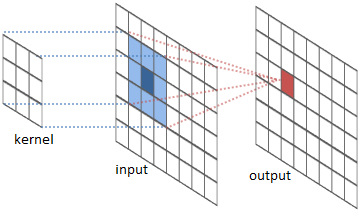
\includegraphics[scale=0.7]{images/kernel_convolution.png}
\end{center}
        \end{enumerate}
\end{enumerate}
    \item \textbf{Pooling layers}: Convolutional layers produce images that have the same width and height as the image the layer recieved (and often with a greater depth, since the outputted image's depth is equal to the number of filters used). Seeing as one of the motivations behind CNNs is to reduce the weight space associated with images of very high resolution, we usually put the output of a convolutional layer through a simple \textbf{pooling layer}, which simply downsamples the produced image, thus lowering its dimensions. This is done by partitioning the image into disjoint rectangles with dimensions, $ r_1 $ by $ r_2 $, of pixel values, which are then mapped onto a single pixel value, thus reducing the image's dimensions by a factor of $ r_1 r_2 $. The function mapping the rectangle pixels onto single values is often a simple non-linearity, such as in \textit{max-pooling}, where the maximum pixel value is used. The idea behind pooling is that we want to preserve the information about which features have been detected, and can discard information about exactly where in the image the feature is in favor of maintaining the feature's relative position with respect to other features.
    \item \textbf{Activation layer}: The output of the convolutional layer is an image matrix; a simple activation function is applied element-wise to each pixel in the image matrix, just as in fully connected networks.
\end{enumerate}
In summary, the basic building blocks of CNNs consist of three layers. First, a convolutional layer applies a set of learned image filters to the whole image (through the convolution operator) to produce an image with the same width and height as the original, but with depth equal to the number of filters used (the transformed image produced by each filter is stacked in the depth dimension of the output image). Next, a pooling layer partitions the image produced by the convolutional layer and merges pixel values in the same partition into a single value, thus downsampling the image in order to reduce dimensions. Finally, an activation layer applies some non-linearity (e.g. sigmoid activation with an additive bias term) to the image to produce a final transformed image. This building block of convolutional-pooling-activation layers can be repeated over and over many times. Finally, the final output of all these building blocks is then fed into a fully connected, normal feedforward neural network.

\begin{center}
    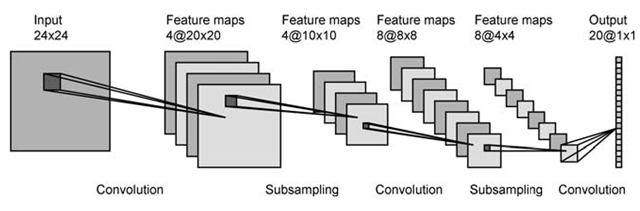
\includegraphics[scale=0.5]{images/conv_net.png}
\end{center}

Let's now mathematically formalize the above ideas by writing the feedforward equations for the CNN, using a stride of one for simplicity. Let $ M $ denote an $ m $ by $ m $ by $ d $ input image matrix (the last dimension is the image depth), and $ p $ be our patch size. If we use $ k $ filters in this layer, let $ W^i $ denote the $ i^{\text{th}} $ filter (i.e. weight matrix), and let $ b $ be the shared $ (n - p) $ by $ (n - p) $ bias matrix. Then the convolutional layer outputs an $ (n - p) $ by $ (n - p) $ by $ k $ matrix which is then passed through an activation layer that applies a non-linearity $ s $ to produce a matrix (with the same dimensions) $ C $, given by
$$ C^i := \text{ $ i^{\text{th}} $ sub-matrix along the depth } = s(b + W^i * M), 1 \leq i \leq k $$
where $ * $ is the convolution operator. The parameters of the convolutional layer are the 3-D tensor $ W $, which contains the $ W^i $'s, and the bias matrix $ b $; these are trained with gradient descent. Next, $ C $ is passed through a pooling layer to reduce the dimensionality of the image. In the pooling layer, we define the pooling factor $ q $ to reduce the size of the images by, and use a pooling function $ P: \mathbb{R}^{q \times q} \rightarrow \mathbb{R} $ to "compress" $ C $ into a new $ \frac{n - p}{q} $ by $ \frac{n - p}{q} $ by $ k $ matrix $ D $, as follows:
$$ D^i_{j, k} = P \left( 
    \begin{bmatrix}
        C^i_{1 + (j - 1) q, 1 + (k - 1) q} & \cdots & C^i_{j q, 1 + (k - 1) q} \\
        \vdots & \ddots & \vdots \\
        C^i_{1 + (j - 1) q, k q} & \cdots & C^i_{j q, k q}
    \end{bmatrix}
\right), 1 \leq i \leq k $$
In other words, we partition $ C^i $ completely into $ q $ by $ q $ sub-matrices, and iteratively pass each one through the pooling function, and put the result in the corresponding spot in the outputted $ \frac{n - p}{q} $ by $ \frac{n - p}{q} $ matrix; we do this for every matrix along the depth, and put it in a corresponding matrix at that depth. The most common choice of $ P $ is simply the $ \max $ function. The outputted image matrix $ D $ can then be used as the input to another convolutional-activation-pooling cycle, or be fed directly into a conventional fully connected network.

\begin{figure}[h]
    \centering
    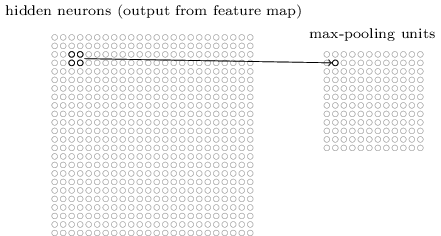
\includegraphics[scale=0.6]{images/conv_net_pooling.png}
    \caption{Example of max-pooling with $ q = 2 $}
\end{figure}
To train the CNN, we can use gradient descent with a few modifications to backpropagation; adapting the algorithm isn't difficult since kernal convolutions are simple differentiable functions, and the only other factors to account for are the pooling function. As in most deep learning paradigms, CNNs learn hierarchically; earlier layers learn to identify simple image features, such as edges, from the original image, while later layer blocks learn to identify more complex features, such as shapes, based on activation maps produced by the earlier layers, which highlight simple features and enable the detection of complex features from simple ones.

\section{Recurrent Neural Networks}
One of the primary assumptions standard neural nets make is that individual training samples are independent of each other. This means that they're not very good at learning sequential data, that is, data in which variable-length sequences of data have patterns which need to be learned, rather than a straightforward mapping of independent inputs to outputs. In particular, time-series data, in which multiple real-valued vectors are each associated with a time stamp, representing a chronological evolution in the data. One of the most salient applications of a model capable of learning time series data is in machine perception; other important examples of time series data include frames of a video (video processing), words in a sentence (NLP), and audio data (music or speech processing).
\newline \newline
In order to modify the neural network model to apply to sequential data, we need to introduce some mechanism of memory, so the network's output depends not only on the input, but on previous inputs as well. This is where recurrent neural networks, or RNNs, come in. RNNs are a type of neural network that follow the same connectionist paradigm but are capable of selectively passing information across training steps. Thus, unlike conventional neural nets, the state isn't lost after a run on an input. As opposed to other models capable of learning sequential data, such as hidden Markov models, RNNs can "remember" information an arbitrary number of time steps in the past with little to no computational overhead, and exploit the high dimensionality of their weight space to represent a sufficiently large state space without becoming computationally infeasible to train. Indeed, the number of possible states that can be represented in a layer of a neural net grows exponentially with the number of nodes in the layer. On the other hand, other models such as HMMs tend to grow quadratically or even exponentially with the size of the state space; since most of the problems mentioned above would require astronomically large state spaces to explicitly represent, this renders most of these models infeasible to train in practice. Training time for neural nets with backpropagation is bounded quadratically in the number of nodes, even though the expressive power scales exponentially, making them a very useful model.
\newline \newline
Because RNNs are an extension of feedforward neural nets, they obey a universal approximation theorem of their own - a finite size RNN with sigmoid activation function can is Turing complete. Moreover, RNNs are completely differentiable and hence can be trained with gradient descent.

\subsection{Architecture}
There are many different architecures available for use in RNNs; let's look at the most basic one. The idea is that we'll start with the standard feedforward graph topology, and augment it with edges capturing state. Specifically, we'll introduce \textit{recurrent edges}, which can be visualized as connecting every node in a hidden layer to every other node (including itself) in the same hidden layer.

\begin{center}
    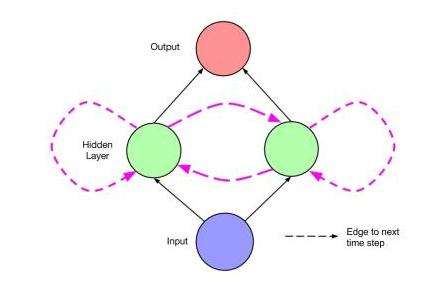
\includegraphics[scale=0.7]{images/rnn.png}
\end{center}

RNNs are designed to accept sequences of input vectors, which we write $ ( x^0, \cdots, x^t, \cdots, x^T ) $, rather than individual input vectors. The recurrent edges capture state. The key is that when passing an input vector forward through the network, a hidden node's output is dependent on both the outputs of the nodes in the previous hidden layer (as in feedforward nets) and the values of the recurrent edges (which are themselves weighted). To formalize this, let's first discuss the architecture of a \textit{simple RNN}, defined as an RNN with a single hidden layer, and then extend it to a \textit{deep RNN}, an RNN with an arbitrary number of hidden layers.

\subsubsection{Simple RNN Architecture}
Suppose we're given an input sequence $ x = (x^{(t)})_{1 \leq t \leq T} $. Let $ f $ be our activation function. The hidden layer is parameterized by three weight matrices: $ W_1 $, the weight matrix between the input layer and the hidden layer, $ W_2 $, the weight matrix between the hidden layer and the output layer, and $ V $, the weight matrix for the recurrent edges. We feed the sequence through the RNN by passing $ x^{(t)} $ through the network at time step $ t $, using the following feedforward equations:
$$ s^{(t)} = \text{ hidden state at time step $ t $ } = f(W_1 x^{(t)}, V s^{(t - 1)}) $$
$$ o^{(t)} = \text{softmax}(W_2 s^{(t)}) $$
What's really happening here is that the hidden layer's output depends not only on the input vector but also on the output of itself from the last time step. What's really going on here is that the hidden nodes are connected not only to the hidden nodes of the next layer but also to hidden nodes in the same layer, at the next time step (as is seen in the dependence of the output of a hidden node on the past state, which is dependent on the output of the same hidden nodes). In other words, hidden nodes in a given layer can "talk" to hidden nodes in the same layer, but in the future. This is visualized by "unrolling" the network, which paints the RNN as multiple copies of a single base feedforward network in which hidden units, in addition to passing information to the next layer, pass information to their counterparts in the next network copy:

\begin{center}
    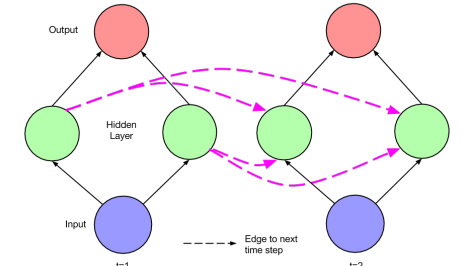
\includegraphics[scale=0.5]{images/unrolled_rnn.png}
\end{center}

\subsubsection{Deep RNN Architecture}
Let's now extend the simple architecture to arbitrarily many layers. The simplest way to do this, for a fixed hidden layer, is to just compute our state as usual, as a function of the weighted output from the previous layer and the weighted state from the last time step, and simply pass the new state for the hidden layer as the output of the hidden layer:
$$ s_i^{(t)} = f(W_i o_{i - 1}^{(t)} + V_i s_i^{(t - 1)}) $$
$$ o_i^{(t)} = s_i^{(t)} $$
where $ W_i $ is the weight matrix between hidden layers $ i - 1 $ and $ i $, and $ V_i $ is the weight matrix for the recurrent edges of layer $ i $. As usual we pass the output of the last hidden layer through a softmax function.
\newline \newline
The connections hidden nodes have to their "future" selves is what allows RNNs to work with sequential data, where the inputs span across multiple consecutive runs of the network. Notice that this makes it possible for the network, which in the feedforward case forms a directed acyclic graph (DAG), to have cycles. However, after unrolling the network, we again have a DAG, albeit a much deeper one, with shared weights, instead of unique weight matrices for each layer, across time steps. We can use backpropagation to train the unrolled network; this modified algorithm is known as \textit{backpropagation through time}, or BPTT. One final note - although the network has an output at every time step, in practice we often only want the network's aggregate output after its seen the entire sequence we want to pass through it, in which case we simply discard all the outputs except the last. The hidden state and recurrent weights together capture the concept of an RNN's memory of past inputs, though in practice RNNs have some trouble remembering or accounting for information and input vectors they saw more than a few time steps in the past.

\subsubsection{Hopfield Architecture}
There are many different RNN architectures, all inspired on the above theory. One of the earliest graph topologies popularized in the 1980s by John Hopfield was a structure in which every node is connected to every other node (except itself), and connections have symmetric weights; in other words, the network is a weighted undirected complete graph. Moreover, nodes are binary threshold units - they only output $ 1 $ or $ -1 $, depending on whether the weighted linear combination of inputs to the node exceeds an associated threshold or not, similar to the very early multilayer perceptron model of feedforward neural nets.
$$ \text{For node } i: s_i = \begin{cases}
    1, &\text{ if } \sum_{j \neq i} w_{i, j} s_j > \theta_i \\
    -1, &\text{ otherwise }
\end{cases} $$
where $ \theta_i $ is the threshold of node $ i $, and $ w_{i, j} $ is the weight between nodes $ i $ and $ j $. The graph is obviously cyclic, and indeed not even directed, so backpropagation simply isn't possible; instead, nodes are updated asynchronously - that is, one by one, with all the weights of a node being updated when it's that node's turn. Usually the order in which nodes are selected to be updated is random.
\newline
Hopfield networks were designed to emulate associative memory - essentially the weights of the network encode a certain set of patterns, and when the network is given a partial pattern or fragment of a pattern, it outputs the corresponding full pattern. This has been successfully applied to the recovery of corrupted data or fuzzy classification. The idea of associative memory is borrowed from neuroscience, referencing the phenomenon in which certain stimuli can quickly evoke anchored memories. In this vein, the (unsupervised) learning algorithm for Hopfield networks is based on Hebbian learning, a theory in neuroscience that can be summarized by the maxim of the mammalian brain that "neurons that fire together wire together". In other words, when two nodes tend to have the same state, the weight between them is strengthened, whereas nodes that tend to have opposite states have decaying weights.

\subsubsection{Jordan Architecture}
Michael Jordan, a professor at UC Berkeley, proposed another early network topology for RNNs in the 1980s. The structure took a feedforward neural net and placed several \textit{context units} alongside the hidden nodes, with the output of the next layer feeding into the context units (unweighted) and the output of the context units feeding into the hidden nodes (weighted) of the next time step. Thus, the hidden nodes see the output of the previous layer as input, just as in a normal feedforward network, but also the output of the context units, which represents the state from the previous time step. 

\begin{center}
    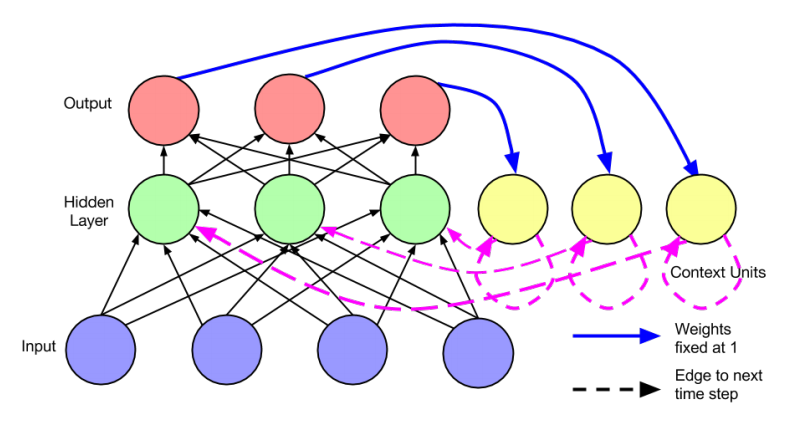
\includegraphics[scale=0.35]{images/jordan_rnn.png}
\end{center}

The context nodes are also self-connected (though not connected to other hidden nods). Jordan networks are most commonly three layers (ie one hidden layer).

\subsubsection{Elman Architecture}
Similar to the Jordan architecture, but the hidden nodes feed back into the context units, instead of the output layer. This is equivalent to the RNN structure we introduced before, where each hidden node has a single recurrent edge to itself. Elman networks are, like Jordan networks, typically three layers deep.

\begin{center}
    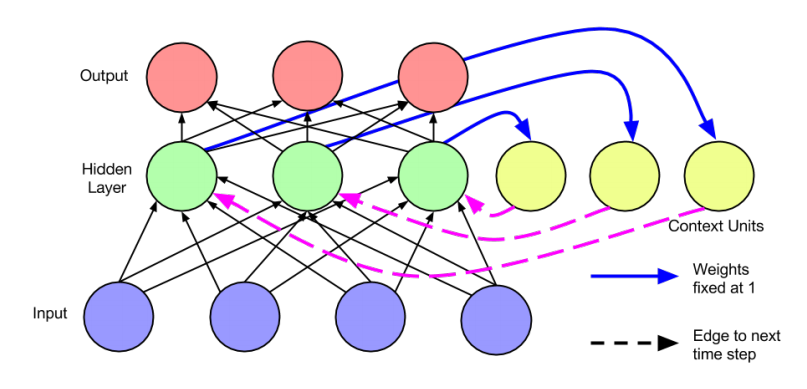
\includegraphics[scale=0.35]{images/elman_rnn.png}
\end{center}

\subsection{Long-Term Short-Term RNNs}
Although in principle an RNN should be able to recall and use information arbitrarily far in the past when it produces an output vector, in practice they just don't seem to learn dependencies more than a few time steps in the past. More commonly known as LSTMs, this model was the first to demonstrably learn even very large time dependencies, many time steps in the past. One of the main reasons it's difficult to train RNNs, and neural networks in general, and also a limiting factor in remembering long term time dependencies, is the vanishing gradient problem. LSTMs introduce a new kind of network node called the \textit{LSTM unit}, which has no activation function for the recurrent edges, and hence isn't subject to the vanishing gradient problem.
\newline
LSTM units have a somewhat complicated structure, so let's break it into its component parts. Like other nodes, LSTM units receive as input both the output vector from the previous layer and the state of the recurrent edges. At any given point, an LSTM unit keeps track of it's own state, $ S $ (not related to the state of recurrent edges). Much like computer memory (though analog instead of digital, to ensure differentiability), the state can be read from, written to, and erased (again, these operations are continuous instead of discrete). These operations are governed with \textit{gates} - LSTM units have an \textit{input gate}, a \textit{forget gate}, and an \textit{output gate}. All three gates receive the same input vectors, namely the output of the last layer, $ o_{i - 1} $, and the layer's current state, $ s_i^t $. 
\newline \newline
\textbf{LSTM Data Flow}: Let's take a detailed look at how information flows through the LSTM unit. All decisions made in the data pipeline are based on the current state of the LSTM and the received input. Starting at each gate, where the input is processed by each gate node (in parallel) as if the gate node were a regular feedforward neural net node - that is, taking a weighted linear combination of the inputs, throwing on a bias term, and passing through an activation function. First, the forget gate uses the processed input to decide how much of the current state to erase, or forget. Next, the input gate uses it to decide how much the received input will influence and be stored in the LSTM state. Finally, the output gate produces a combination of a filtered version of the LSTM's (now updated) state and the processed input. Below, we use $ W $ to stand for the weight matrices, and $ \theta $ for the bias terms, for each of the gates. 
\begin{enumerate}
    \item \textbf{Input processing}: All of the operations are done with a concatenated version of the recurrent state and previous layer output, which we use as the input $ I $ to the LSTM input.
$$ I = \begin{bmatrix} o_{i - 1} & s_i^t \end{bmatrix} $$
\item \textbf{Forget gate}: The forget gate produces a value $ f_1 $ between zero and one, representing how much to weight the current state, or at a higher level how much to forget.
$$ f_1 = \sigma(W_{\text{forget}} \cdot I + \theta_{\text{forget}}) $$
    \item \textbf{Input gate}: Simultaneously, the input gate choose creates a its own candidate input $ c $ from the recurrent state and previous layer outputs.
$$ c = \sigma(W_{\text{input}} \cdot I + \theta_{\text{input}}) $$
as well as a value $ f_2 $ between zero and one, representing how much to weight the current state:
$$ f_2 = \sigma(W_{\text{input}} \cdot I + \theta_{\text{input}}) $$
We can then update the state $ S $ as a mixture of what's already stored and the new information the unit just saw:
$$ S \gets f_1 S + f_2 c $$
    \item \textbf{Output processing}: Finally, we need to figure out what the unit will output. This is handled by the output gate, which simply outputs the product of the unit's (updated) internal state and the processed input.
$$ f_3 = \sigma(W_{\text{output}} \cdot I + \theta_{\text{input}}) $$
$$ o = f_3 \sigma(S) $$
\end{enumerate}
Although we used $ \sigma $ throughout the above to denote the activation function, it's common for $ c $ and $ o $ to use different activation functions (usually hyperbolic tangent, whereas the original $ \sigma $ is usually sigmoid).

\begin{center}
    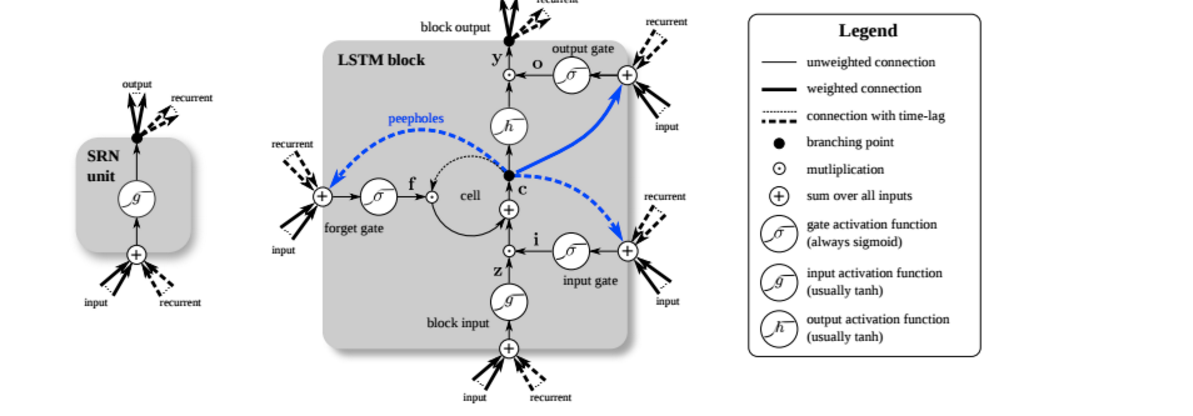
\includegraphics[scale=0.4]{images/lstm_diagram.png}
\end{center}

The LSTM is therefore more like a combination of several parallel feedforward layers that determine how to save, erase, read from, and write to a persistent analog state - this is what allows LSTM units to remember information arbitrary time steps in the past. This is very much in part due to the fact that LSTM units don't iteratively squash the gradient and so don't suffer from the vanishing gradient problem. Instead, when error values are backpropagated to LSTM units, the unit traps the error by iteratively feeding the error signal back into each gate until the gates learn to cut off the error signal.
\newline \newline
In practice, there are many variations of the standard LSTM unit that are used. For example, it's common to sometimes allow the gates to use the current LSTM state, in addition to the inputs and recurrent state, in processing; such units are called \textit{peephole LSTMs}. Sometimes a convolution operator is used instead of multiplication (this is known as a \textit{convolutional LSTM}). Yet another variation is to combine the input and forget gates, using a single forget weighting and one minus that weight for the input weighting instead of separate forget and input weightings. This is based on the intuitive notion that we only want to forget things when we're adding new things; otherwise, there's no reason to destroy information. One popular modern approach is called the \textit{gated recurrent unit}, or GRU, which is a simplified version of the LSTM in which forget and input gates are combined as described above, but recurrent state and LSTM state are also merged into a single state. Moreover, GRUs have no output gate, instead simply outputting its unweighted state.

\subsubsection{Encoder-Decoder Models}
RNNs have the primary advantage of being able to learn sequential data, and ideally we'd like to formulate a recurrent architecture capable of handling arbitrary length sequential inputs and outputs. Let's take a look at one common network architecture that makes minimal assumptions on the structure of the sequential training data. Our approach is end-to-end differentiable, and makes use of a multi-layer RNN with LSTM units to first encode input vector sequences, one element per time step, to a vector representation of fixed dimensionality, followed by another deep LSTM RNN network to decode the target sequence from the vector representation. LSTMs are useful because of their practical ability to learn long-term time dependencies, since there might be a significant time lag between elements of the input sequence that map to the corresponding elements in the output sequence.
\newline
TODO

https://papers.nips.cc/paper/5346-sequence-to-sequence-learning-with-neural-networks.pdf

\subsection{Bidirectional RNNs}
    The other major variant of standard RNNs that used in practice today is the BRNN. The guiding principle is that RNNs only have access to past data, but not future data. BRNNs have two parallel hidden layers, one with recurrent edges to the state at the previous time step (as with normal RNNs), and one with recurrent edges to the next time step. The hidden nodes of the network are thus partitioned into a positive time direction and a negative time direction. Of course, the major flaw in this design is that BRNNs can't run online (processing and learning data point by data point in real time) since they require access to the entire sequence at once. The defining equations of a BRNN, where we denote the forward time state of layer $ i $ with $ s_i^{t+} $ and the backward time state of layer $ i $ with $ s_i^{t-} $, are
$$ \begin{aligned}
    s_i^{t+} &= \sigma \left( W_{i - 1}^+ o_{i - 1} + V_i^+ s_i^{(t - 1)+} \right) \\
    s_i^{t-} &= \sigma \left( W_{i - 1}^- o_{i - 1} + V_i^- s_i^{(t + 1)+} \right) \\
    o_i &= W_i^+ s_i^{t+} + W_i^- s_i^{t-}
\end{aligned} $$
$ W_i^+ $ and $ W_i^- $ are the weights from layer $ i $ to layer $ i + 1 $, in the forward and backward time directions respectively, and $ o_i $ is the output of layer $ i $. As with regular RNNs, the softmax function is often applied to the last layer, and usually only a single pair of forward and backward time hidden layers is used. BRNNs can be unrolled across all time steps (ie over the full sequence), and then trained with backpropagation. Some have tried combining BRNNs with LSTMs, using LSTM units as nodes in a BRNN graph topology.

\end{document}
